\documentclass[a4paper,11pt]{article}
\usepackage{amsmath, amssymb, graphicx, siunitx, subcaption, float, booktabs}
\usepackage[margin=1.5cm]{geometry}  % margins set to 1.5 cm
\usepackage{titlesec}
\usepackage{physics}
\usepackage{xcolor}
\usepackage{caption}

\title{\textbf{Lumped Element Matching Netwrok Design}}
\author{Amirkahshayar Maghsoud}
\date{}
\begin{document}

\maketitle
\section{Introduction}

The following data have been used in the calculations. They are taken from the data provided for $F=1$ in Homework~No.~2:

\begin{center}
\begin{tabular}{cc}
$Z_C = 50~\Omega$ & $Z_L = 533~\Omega$ \\[6pt]
$f_0 = 1953~\text{MHz}$ & $y_L = \dfrac{1}{Z_L} = 0.0938~\text{S}$
\end{tabular}
\end{center}


\section{Lumped Element Matching Network}

In this section, the circuit topology shown in the lecture slides has been selected, since the normalized impedance $Z_L/Z_0$ lies inside the $1 + jx$ circle of the Smith chart, or equivalently
$\Re\{Z_L\} > Z_C$.
The following results correspond to the two matching solutions obtained using a single shunt stub adaptor.

\subsection*{Matching Using a Single Shunt Stub}

\begin{itemize}
    \item $D_{\text{stub},1} = 31.115~\text{mm}$
    \item $l_{\text{stub},1} = 7.963~\text{mm}$
    \item $D_{\text{stub},2} = 45.637~\text{mm}$
    \item $l_{\text{stub},2} = 68.789~\text{mm}$
\end{itemize}

\subsection*{Matching Using Lumped Elements}

In this subsection, the values of the susceptance $B$ and the reactance $X$ are calculated using the formulas given below.
The matching network consists of a series reactance $jX$ and a shunt susceptance $jB$, realized using the components
$C_1$, $L_1$, $C_2$, and $L_2$.

\subsubsection*{Lumped Element Matching Network Solutions}

\begin{equation}
\begin{aligned}
B_1 &=
\frac{
X_L + \sqrt{\frac{R_L}{Z_0}}
\sqrt{R_L^2 + X_L^2 - Z_0 R_L}
}{
R_L^2 + X_L^2
}
= 0.0058~\text{S}, &
B_2 &=
\frac{
X_L - \sqrt{\frac{R_L}{Z_0}}
\sqrt{R_L^2 + X_L^2 - Z_0 R_L}
}{
R_L^2 + X_L^2
}
= -0.0058~\text{S} \\[6pt]
X_1 &=
\frac{1}{B_1}
+ \left( \frac{X_L Z_0}{R_L} \right)
- \left( \frac{Z_0}{B_1 R_L} \right)
= 155.4027~\Omega, &
X_2 &=
\frac{1}{B_2}
+ \left( \frac{X_L Z_0}{R_L} \right)
- \left( \frac{Z_0}{B_2 R_L} \right)
= -155.4027~\Omega \\[6pt]
C_1 &= \frac{B_1}{2\pi f_0} = 4.7520 \times 10^{-13}~\text{F}, &
C_2 &= -\frac{1}{2\pi f_0 X_2} = 5.2440 \times 10^{-13}~\text{F} \\[6pt]
L_1 &= \frac{X_1}{2\pi f_0} =1.2664 \times 10^{-8}~\text{H}, &
L_2 &= -\frac{1}{2\pi f_0 B_2} = 1.3975 \times 10^{-8}~\text{H}
\end{aligned}
\end{equation}


\section{Plots of the Matching Networks}

\subsubsection*{Single-Stub Matching Network (2 Solutions)}

\begin{figure}[H]
\centering
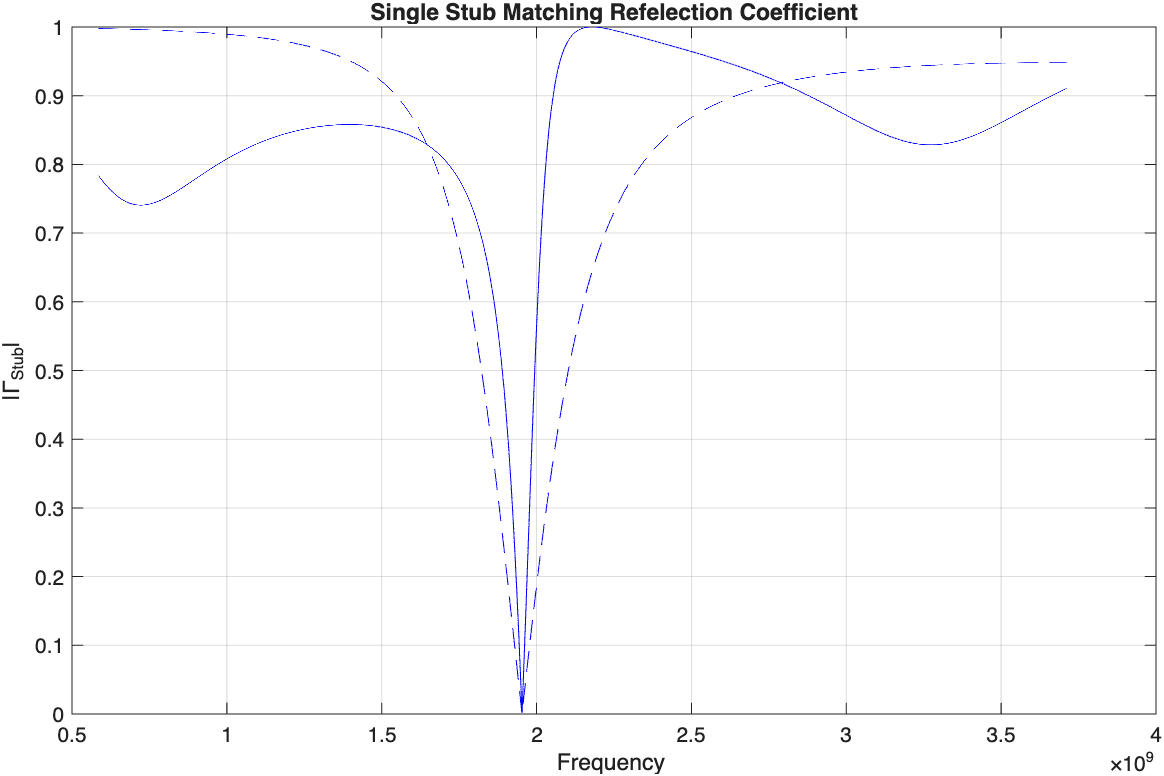
\includegraphics[width=0.6\linewidth]{sinlgestub.png}
\caption{Reflection coefficient magnitude for the single-stub matching network.}
\end{figure}

\subsubsection*{Lumped-Element Matching Network (2 Solutions)}

\begin{figure}[H]
\centering
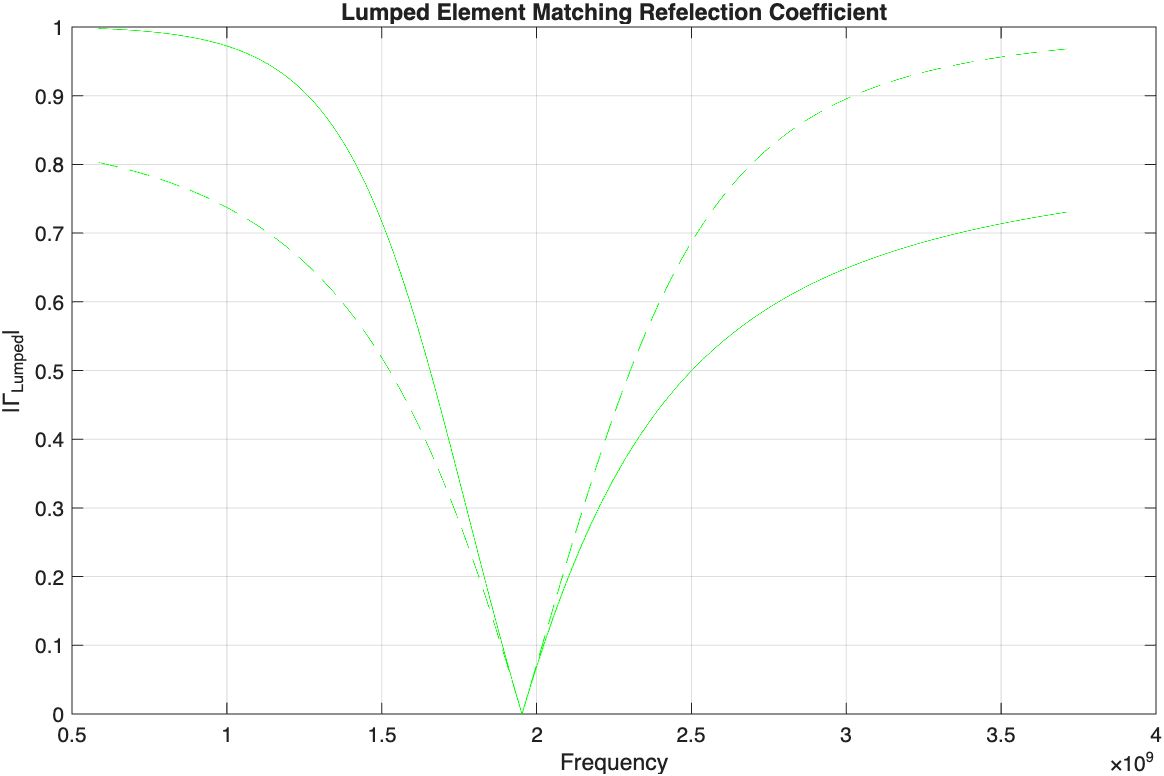
\includegraphics[width=0.6\linewidth]{lumpedmatching.png}
\caption{Reflection coefficient magnitude for the lumped-element matching network.
}
\end{figure}

\section{Bandwidth for $\Gamma_m < 0.025$}

The estimated bandwidths for the different matching networks are summarized below:

\[
\begin{aligned}
\text{Single-stub matching (Solution 1)} &: 11.563~\text{MHz},\\
\text{Single-stub matching (Solution 2)} &: 4.0626~\text{MHz},\\
\text{Lumped-element matching (Solution 1)} &: 32.814~\text{MHz},\\
\text{Lumped-element matching (Solution 2)} &: 32.814~\text{MHz}.
\end{aligned}
\]

\section{Multisection Transformer}

\subsection*{Three-Section Transformer}

Let the source and load impedances be
\[
Z_0 = 50~\Omega, \quad Z_L = 533~\Omega
\]

For $N = 3$, the equation for impedances is:
\[
\ln\frac{Z_{n+1}}{Z_n} = 2^{-N} C_n^N \ln \frac{Z_L}{Z_0}
\]

The binomial coefficients for $N = 3$ are:
\[
C_3^0 = 1, \quad C_3^1 = 3, \quad C_3^2 = 3, \quad C_3^3 = 1
\]

Calculating the impedances:

\[
Z_1 = \left(\frac{Z_L}{Z_0}\right)^{1/8} Z_0 = 67.2109~\Omega, \quad
Z_2 = \left(\frac{Z_L}{Z_0}\right)^{3/8} Z_1 = 163.2483~\Omega, \quad
Z_3 = \left(\frac{Z_L}{Z_0}\right)^{3/8} Z_2 = 396.5131~\Omega
\]

Reflection coefficients:

\[
\Gamma_0 = 0.147, \quad
\Gamma_1 = 0.4165, \quad
\Gamma_2 = 0.4168, \quad
\Gamma_3 = 0.147
\]

From the obtained reflection coefficients, since $\Gamma_0 = \Gamma_3 = 0.147$, it can be concluded that the calculated impedance values $Z_1$ to $Z_3$ are correct and symmetric with respect to the source and load.

\subsubsection*{Summary of Three-Section Transformer:}
\[
Z_0 = 50~\Omega, \quad Z_1 = 67.211~\Omega, \quad Z_2 = 163.248~\Omega, \quad Z_3 = 396.513~\Omega, \quad Z_L = 533~\Omega
\]



\subsection*{Four-Section Transformer}

For $N = 4$, the binomial coefficients are:
\[
C_4^0 = 1, \quad C_4^1 = 4, \quad C_4^2 = 6, \quad C_4^3 = 4, \quad C_4^4 = 1
\]

Calculating the impedances:

\[
Z_1 = \left(\frac{Z_L}{Z_0}\right)^{1/16} Z_0 = 57.9702~\Omega, \quad
Z_2 = \left(\frac{Z_L}{Z_0}\right)^{4/16} Z_1 = 104.7476~\Omega
\]

\[
Z_3 = \left(\frac{Z_L}{Z_0}\right)^{6/16} Z_2 = 254.4211~\Omega, \quad
Z_4 = \left(\frac{Z_L}{Z_0}\right)^{4/16} Z_3 = 459.7189~\Omega
\]

Reflection coefficients:

\[
\Gamma_0 = 0.0738, \quad
\Gamma_1 = 0.2874, \quad
\Gamma_2 = 0.4166, \quad
\Gamma_3 = 0.2874, \quad
\Gamma_4 = 0.0738
\]

From the obtained reflection coefficients, the symmetry
$\Gamma_0 = \Gamma_4$ and $\Gamma_1 = \Gamma_3$
confirms the correctness of the calculated impedance values for the
four-section transformer.

\subsubsection*{Summary of Four-Section Transformer:}
\[
Z_0 = 50~\Omega, \quad Z_1 = 57.970~\Omega, \quad Z_2 = 104.748~\Omega, \quad Z_3 = 254.421~\Omega, \quad Z_4 = 459.719~\Omega, \quad Z_L = 533~\Omega
\]


\section{Plots of the Multisection Transformer}

The $N$-section matching network and the reference transmission line
are modeled using ABCD matrices.
For a transmission line section with characteristic impedance $Z_n$
and electrical length $\beta l$, the ABCD matrix is given by
\[
\mathbf{A}_n =
\begin{bmatrix}
\cos(\beta l) & j Z_n \sin(\beta l) \\
j \dfrac{\sin(\beta l)}{Z_n} & \cos(\beta l)
\end{bmatrix},
\qquad n = 1,\dots,N.
\]

The reference transmission line with characteristic impedance $Z_0$
and length $l_0$ is described by
\[
\mathbf{A}_0 =
\begin{bmatrix}
\cos(\beta l_0) & j Z_0 \sin(\beta l_0) \\
j \dfrac{\sin(\beta l_0)}{Z_0} & \cos(\beta l_0)
\end{bmatrix}.
\]

For the case $N=4$, the overall ABCD matrix of the cascaded network is
\[
\mathbf{A}_{\text{tot}} =
\mathbf{A}_1 \mathbf{A}_2 \mathbf{A}_3 \mathbf{A}_4 \mathbf{A}_0.
\]

\subsection*{Case $N=3$}

The figure below compares the estimated and exact solutions for the
three-section matching network. The estimated solution is represented by the
red dashed curve, while the exact solution obtained using the ABCD matrix
formulation is shown by the solid blue curve.

\begin{figure}[H]
\centering
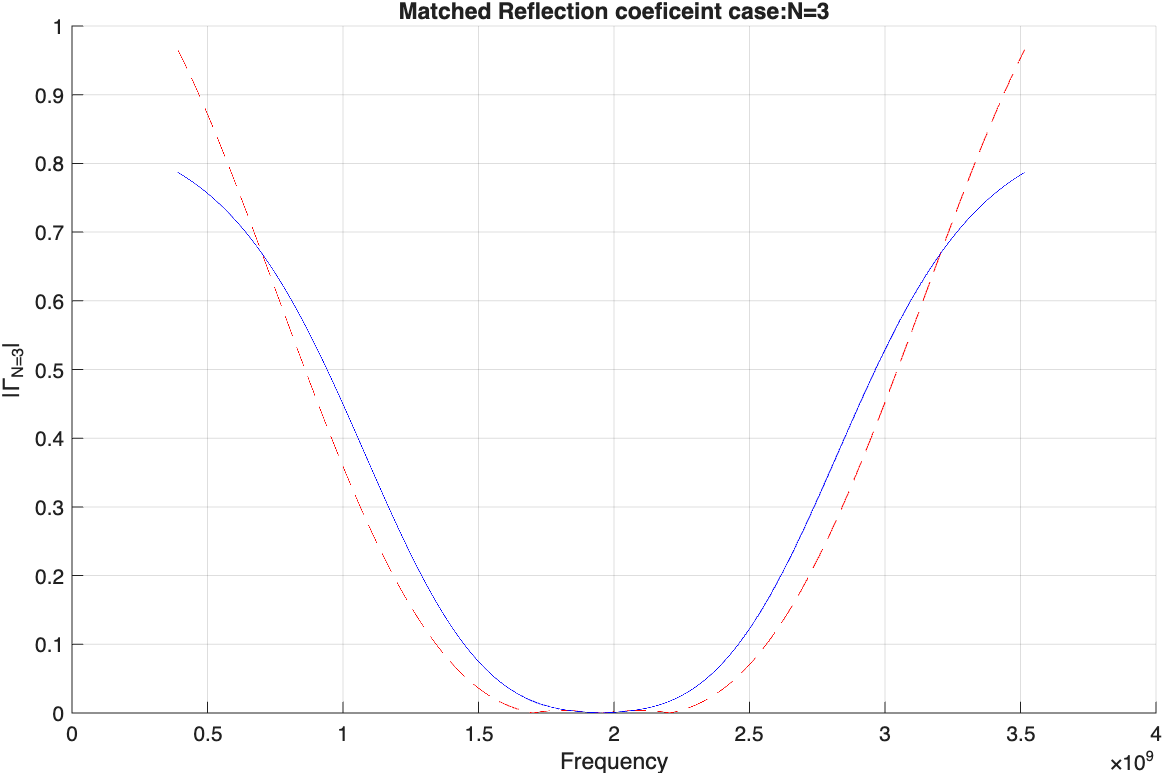
\includegraphics[width=0.6\linewidth]{gaman3.png}
\caption{Reflection coefficient magnitude for the three-section maximum-flat transformer.}
\end{figure}

\subsection*{Case $N=4$}

The figure below shows the reflection coefficient magnitude for the
four-section matching network. The estimated and exact solutions are
represented similarly.

\begin{figure}[H]
\centering
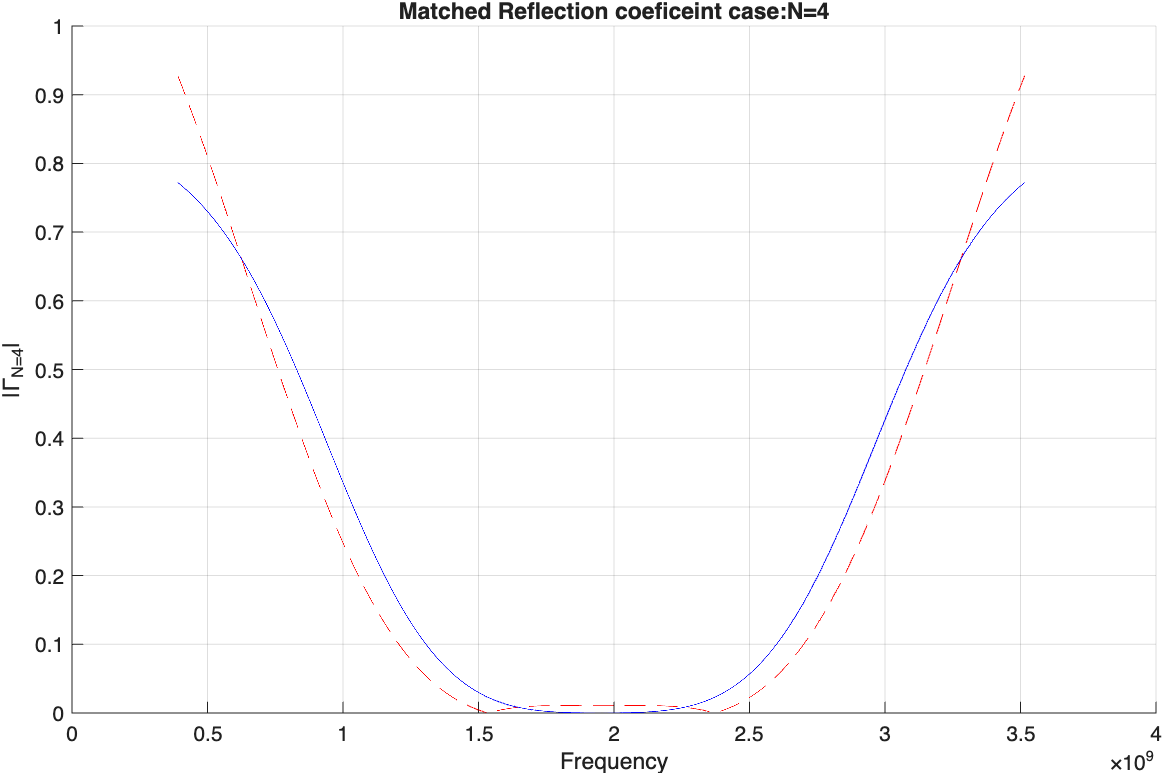
\includegraphics[width=0.6\linewidth]{gamman4.png}
\caption{Reflection coefficient magnitude for the four-section maximum-flat transformer.}
\end{figure}

\section{Estimated Bandwidth of Maximum-Flat Multisection Transformers}

The estimated bandwidths for the three-section and four-section
maximum-flat matching transformers are summarized below:

\begin{equation}
\begin{aligned}
A_3 &= 2^{-3}\frac{Z_L - Z_0}{Z_L + Z_0} = 0.1035,
&
A_4 &= 2^{-4}\frac{Z_L - Z_0}{Z_L + Z_0} = 0.05177
\\[8pt]
\frac{B_3}{f_0} &=
2 - \frac{4}{\pi}
\cos^{-1}
\left[
\frac{1}{2}
\left(
\frac{\Gamma_m}{|A_3|}
\right)^{\frac{1}{3}}
\right]
= 0.4031,
&
\frac{B_4}{f_0} &=
2 - \frac{4}{\pi}
\cos^{-1}
\left[
\frac{1}{2}
\left(
\frac{\Gamma_m}{|A_4|}
\right)^{\frac{1}{4}}
\right]
= 0.5474
\\[8pt]
B_3 &= 787.404~\text{MHz} \quad (f_0 = 1953~\text{MHz}),
&
B_4 &= 1069.08~\text{MHz} \quad (f_0 = 1953~\text{MHz})
\end{aligned}
\end{equation}

\section{Exact Bandwidth of Maximum-Flat Multisection Transformers}

\begin{equation}
\begin{aligned}
B_{3,\text{exact}} &= 589.08~\text{MHz},
&
B_{4,\text{exact}} &= 858.48~\text{MHz}
\end{aligned}
\end{equation}

\section{$\pm6\%$ Random Variation of Impedances in the Matching Network}

This section considers the frequency variation in the range
$0.3 f_0 < f < 1.9 f_0$ for an ensemble of 25 samples of the matching network.
A four-section transformer ($N=4$) is analyzed, where each section impedance
is subject to a random variation of $\pm6\%$.

This corresponds to a multiplicative variation factor in the range
$0.94$ to $1.06$ of the nominal impedance value.

The impedance variation is modeled as
\[
Z_{\text{var}} = Z \,(1 + \delta), 
\qquad \delta \in [-0.06,\, +0.06].
\]

\begin{figure}[H]
\centering
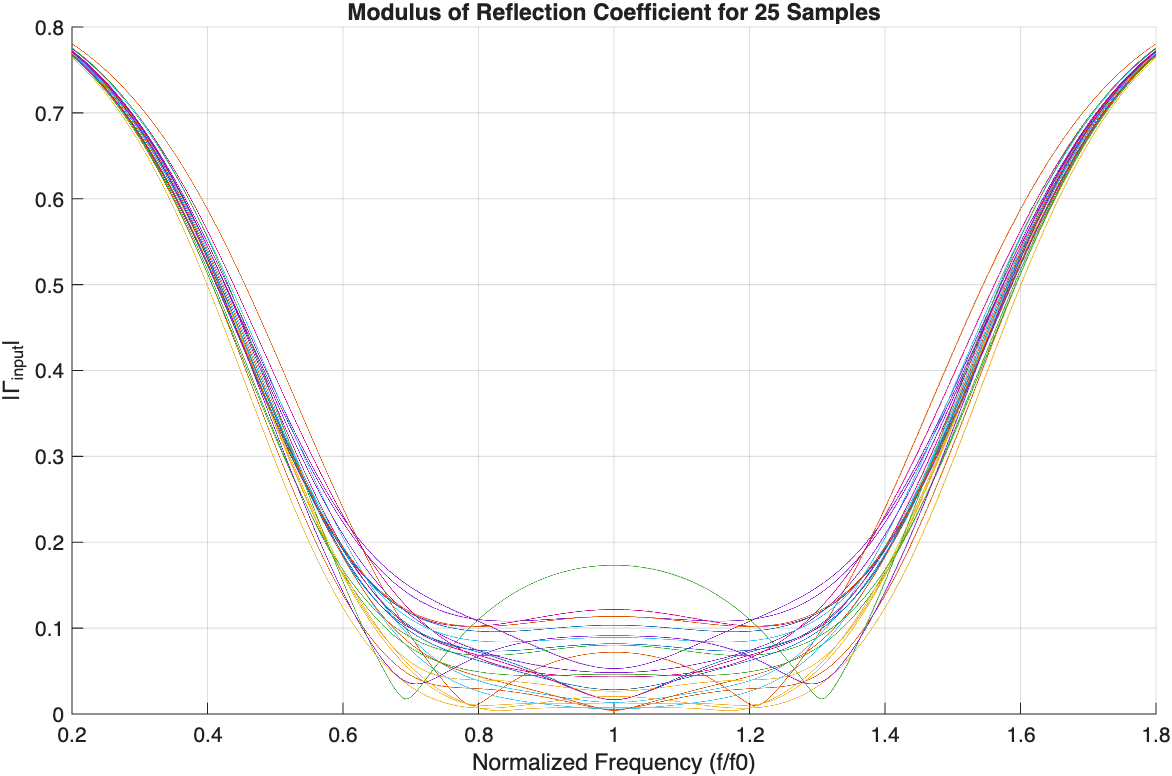
\includegraphics[width=0.6\linewidth]{25smaple.png}
\caption{Reflection coefficient magnitude for the four-section maximum-flat transformer with $\pm6\%$ random impedance variation.}
\end{figure}

\end{document}